\chapter{Dasar Teori}
\label{chap:dasar_teori}

\section{MySQL Spatial Extensions}
\label{sec:mysql_spatial_ex}
	Suatu \textit{geographic feature}\cite{mysqlspatial} adalah sesuatu yang ada di bumi yang memiliki lokasi sebagai penunjuk letak keberadaannya. Geometri adalah cabang ilmu matematika yang digunakan untuk memodelkan suatu \textit{geographic feature}. Dengan geometri, suatu \textit{geographic feature} dapat dinyatakan sebagai sebuah titik, garis, ruang, ataupun bentuk lainnya. Suatu ``\textit{feature}'' yang dimaksud dalam istilah \textit{geographic feature} dapat berupa:
	\begin{enumerate}
		\item \textbf{\textit{An entity}}, contohnya adalah gunung, kolam, kota, dll.
		\item \textbf{\textit{A space}}, contohnya adalah daerah, cuaca, dll.
		\item \textbf{\textit{A definable location}}, contohnya adalah persimpangan jalan, yaitu suatu tempat khusus dimana terdapat 2 buah jalan yang saling berpotongan.
	\end{enumerate}
	
	MySQL adalah salah satu perangkat lunak yang digunakan untuk mengatur data-data (\textit{database}) suatu situs web. Bentuk MySQL adalah sekumpulan tabel-tabel yang umumnya memiliki hubungan antar satu dengan yang lainnya. Setiap tabel pada MySQL memiliki kolom dan baris. Kolom pada MySQL menyatakan daftar jenis baris yang ingin dibuat dan baris menyatakan banyaknya data yang ada dalam tabel.
	
	Penamaan suatu kolom dalam MySQL membutuhkan penentuan jenis tipe data yang akan digunakan dalam kolom tersebut. Dalam MySQL terdapat tipe-tipe data yang umum digunakan seperti \textit{Varchar} untuk menyimpan karakter atau kata, \textit{Int} untuk menyimpan angka, \textit{Boolean} untuk menyimpan nilai ``\texttt{true}'' atau ``\texttt{false}'', dan tipe data lainnya. MySQL Spatial Extensions adalah perluasan dari tipe-tipe data yang disediakan MySQL untuk menyatakan nilai geometri dari suatu \textit{geographic feature}.
	
\subsection{Tipe Data Spatial}
\label{sec:tipe_data_spatial}
Berdasarkan kemampuan penyimpanan nilai geometri\cite{spatialtipedata}, tipe data spatial dapat dikelompokan ke dalam 2 jenis:
\begin{enumerate}
	\item Tipe data yang hanya dapat menyimpan sebuah nilai geometri saja, yaitu:
	\begin{itemize}
		\item \textbf{\textit{Geometry}}
		\item \textbf{\textit{Point}}
		\item \textbf{\textit{LineString}}
		\item \textbf{\textit{Polygon}}
	\end{itemize}
	\item Tipe data yang dapat menyimpan sekumpulan nilai geometri, yaitu:
	\begin{itemize}
		\item \textbf{\textit{MultiPoint}}
		\item \textbf{\textit{MultiLineString}}
		\item \textbf{\textit{MultiPolygon}}
		\item \textbf{\textit{GeometryCollection}}
	\end{itemize}
\end{enumerate}

\subsubsection{\textit{Point}}
\label{sec:point}
\textit{Point} adalah nilai geometri yang merepresentasikan sebuah lokasi ke dalam suatu koordinat\cite{spatialtipedatapoint}. Koordinat pada \textit{Point} terdiri dari nilai X dan Y dimana X merepresentasikan letak lokasi dalam garis bujur dan Y merepresentasikan letak lokasi dalam garis lintang. \textit{Point} tidak memiliki dimensi maupun nilai batasan. Contoh representasi \textit{Point} adalah Universitas Katolik Parahyangan direpresentasikan dalam koordinat X=-6.874735 dan Y=107.6049079 pada skala tertentu (gambar \ref{fig:2_UNPAR}).

\begin{figure}[htbp]
	\centering
		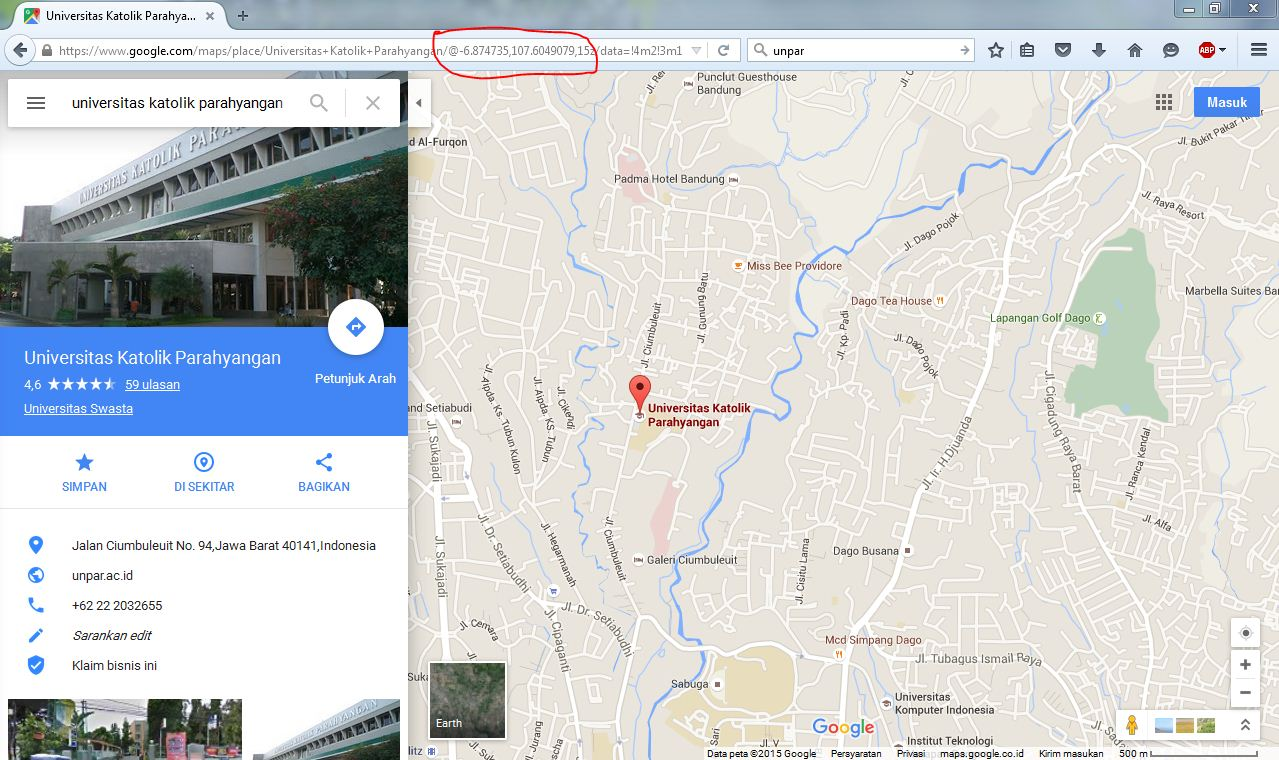
\includegraphics[scale=0.4]{Gambar/2_UNPAR.JPG}
	\caption{Koordinat lokasi Universitas Katolik Parahyangan (\textbf{lingkaran merah})}
	\label{fig:2_UNPAR}
\end{figure}

\subsubsection{\textit{LineString}}
\label{sec:linestring}
\textit{LineString} adalah garis yang terbentuk dari sekumpulan \textit{Point}\cite{spatialtipedatalinestring}. Dalam peta dunia, \textit{LineString} dapat merepresentasikan sebuah sungai dan dalam peta perkotaan, \textit{LineString} dapat merepresentasikan sebuah jalan (contoh: gambar \ref{fig:2_linestring}). Karena \textit{LineString} merupakan sekumpulan \textit{Point}, maka \textit{LineString} menyimpan sekumpulan koordinat dimana setiap koordinat ($X_{1}$..$X_{n}$ dan $Y_{1}$..$Y_{n}$, dimana n menyatakan banyaknya \textit{Point} dalam \textit{LineString}) terhubung oleh garis dengan koordinat selanjutnya. Contohnya: misal terdapat sebuah \textit{LineString} yang mengandung 3 buah \textit{Point}, maka terdapat garis yang menghubungkan \textit{Point} pertama dengan \textit{Point} kedua dan \textit{Point} kedua dengan \textit{Point} ketiga.

\begin{figure}[htbp]
	\centering
		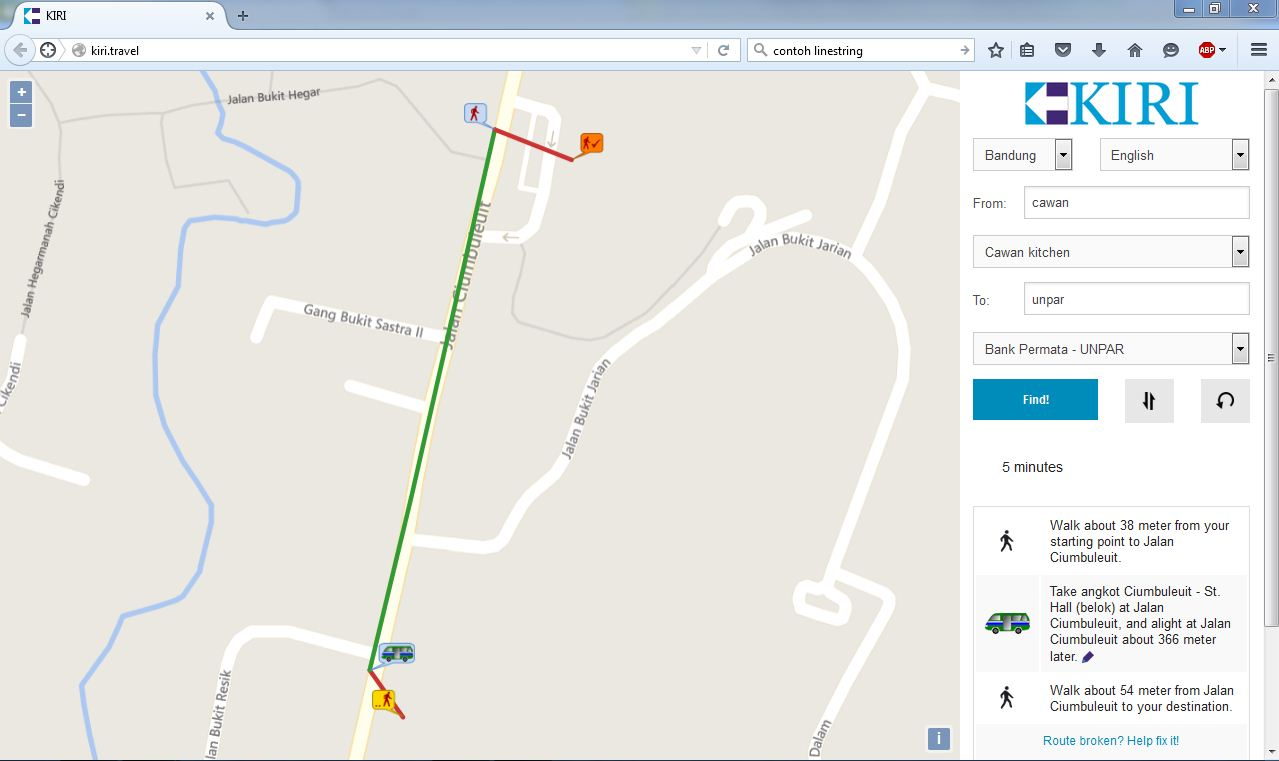
\includegraphics[scale=0.4]{Gambar/2_LineString.JPG}
	\caption{Rute (jalan) yang harus ditempuh dari Cawan Kitchen untuk sampai ke Universitas Katolik Parahyangan direpresentasikan dengan \textit{LineString} (\textbf{garis hijau} dan \textbf{garis merah})}
	\label{fig:2_linestring}
\end{figure}

\section{Play Framework}
\label{sec:play_framework}
Play Framework adalah sekumpulan kerangka kode yang dapat digunakan untuk membangun suatu situs web. Play Framework tidak hanya menggunakan bahasa Java dalam pembuatannya. Bahasa Scala juga digunakan Play Framework dalam beberapa bagian seperti bagian \textit{view} dan \textit{route}\cite{playforjava}. Play Framework menggunakan konsep MVC (\textit{Model} \textit{View} \textit{Controller}) sebagai pola arsitekturnya. Konsep MVC pada suatu kode membuat kode mudah dikembangkan baik secara tampilan maupun pengembangan fitur-fiturnya.

\section{Struktur Aplikasi}
\label{sec:struktur_aplikasi}
Ketika Play Framework pertama kali ter-\textit{install} pada komputer, Play Framework menyediakan \textit{default} direktori dengan struktur minimal (gambar \ref{fig:2_strukturplay}).

\begin{figure}[htbp]
	\centering
		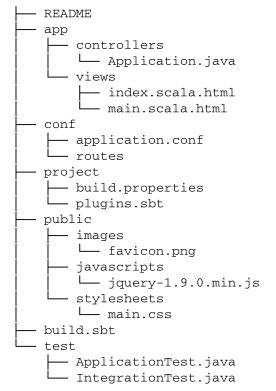
\includegraphics[scale=0.7]{Gambar/2_strukturplay.JPG}
	\caption{Struktur minimal Play Framework}
	\label{fig:2_strukturplay}
\end{figure}




